\documentclass[10 pt]{beamer}
\usetheme{Madrid}
\usepackage[utf8]{inputenc}
\usepackage{xspace}
\usepackage{graphicx,graphics} 
\usepackage{color}
\usepackage{amsmath}
\usepackage{amsfonts}
\usepackage{amssymb}
\usepackage{amsthm}
\usepackage{tabularx}
\usepackage{algorithm}
\usepackage{algorithmic}
\usepackage{longtable}
\usepackage{complexity}
\usepackage{tkz-graph}
\usepackage{float}
\usepackage{multicol}
\usepackage{setspace}
\usepackage[absolute,overlay]{textpos}
\graphicspath{{fig/}}

\tikzset{
  LabelStyle/.style = { rectangle, rounded corners, draw,
                       font = \bfseries },
  EdgeStyle/.append style = {-} }
\title{ Deterministic architectures for low latency in 5G and beyond systems}

\author{{\bf Maël~Guiraud}}


\institute[Nokia Bell Labs, DAVID-UVSQ] 
{
  Nokia Bell Labs France - DAVID, Universit\'e de Versailles Saint Quentin
   \\
}

\subject{Theoretical Computer Science}

\begin{document}


\begin{frame}

  \titlepage
  \centering
  Thesis Supervisor : Dominique Barth\\
   Co-supervisor : Yann Srozecki\\
  
\includegraphics [width=25mm]{logon.png} \hspace{1cm} 
\includegraphics [width=17.5mm]{logod.png} \\
\end{frame}




\begin{section}{Introduction}


\begin{frame}{Use case: Cloud-RAN}
  \centering
  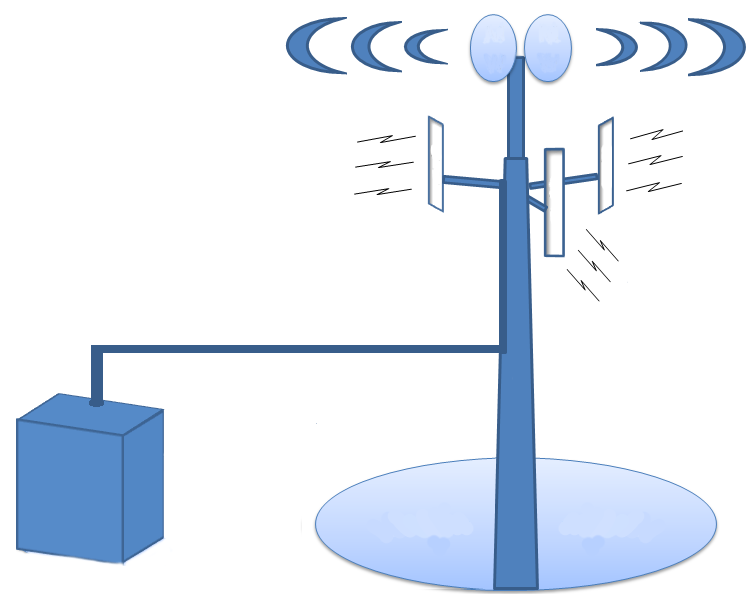
\includegraphics[scale=0.2]{cloudbts.png}\\
  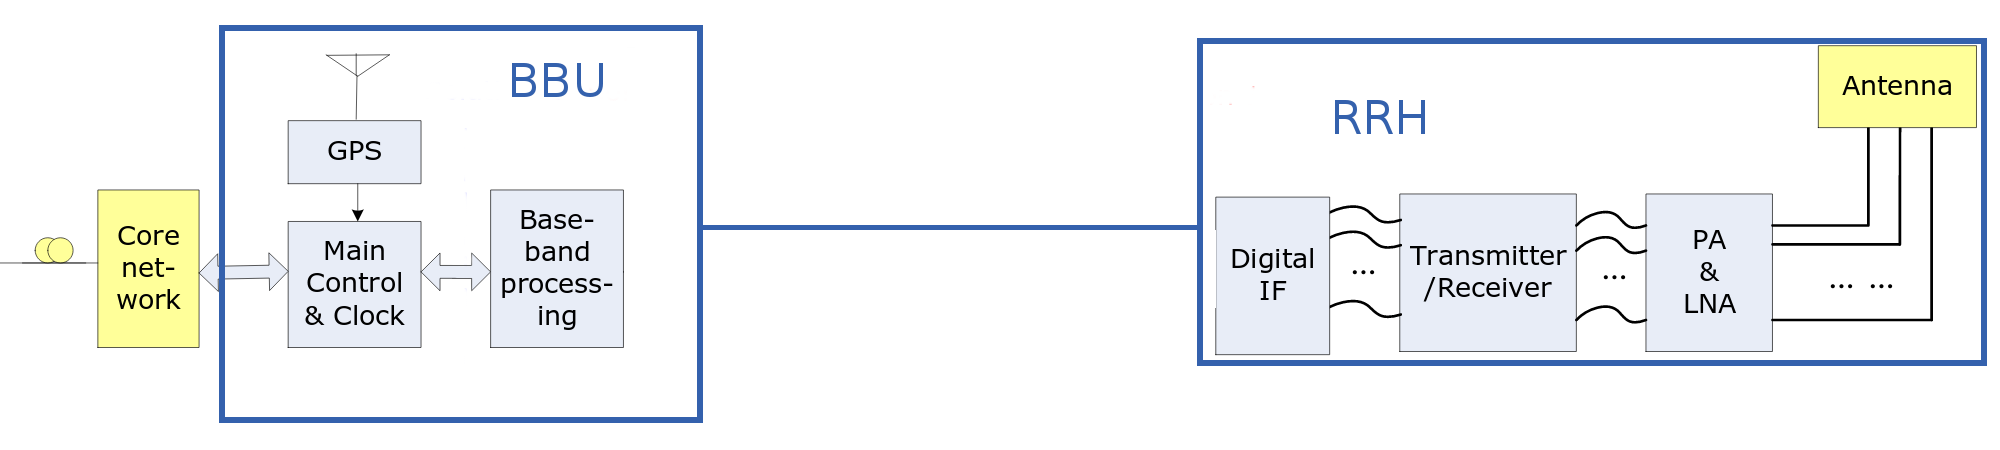
\includegraphics[scale=0.175]{BBURRH.png}
  
   RU=RRH, Distributed/Centralized Unit=BBU
\end{frame}



\begin{frame}{Use case: Cloud-RAN}
  \centering
  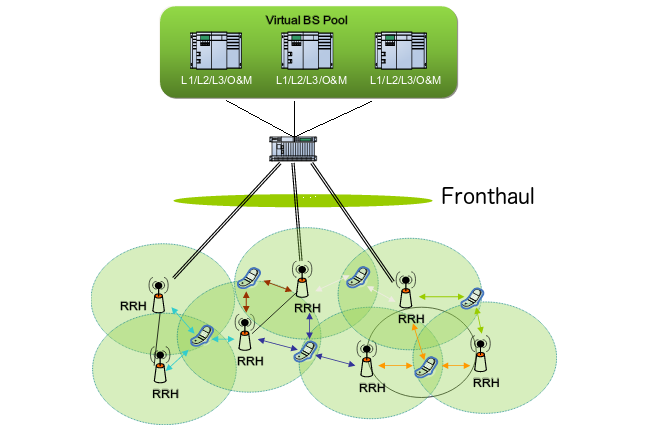
\includegraphics[scale=0.3]{CRAN}\\
  \vspace{0.5cm}
  \pause
  C-RAN aims to mutualize the computation ressources.
  
  \textcolor{red}{Since the processing time is constrained by protocol, the lower the transmission delay, the more important the sharing (ie. the coverage area of a data center).}
  
  \textcolor{blue}{The minimum latency allows to increase the mutualization.}
  
  
\end{frame}


\begin{frame}{Problematic}
  \centering
  
  
 \begin{multicols}{2}
Specificity of Cloud-RAN:
\vspace{1cm}
\begin{itemize}
\item \textcolor{red}{Minimize latency}: increase the cover area.
\item Periodic traffic 

\end{itemize}
\vspace{2cm}
Current approaches: \begin{itemize}
\vspace{1cm}
\item Dedicated network $\rightarrow$ Too expensive
\item Statistical multiplexing (TSN/Qbv) $\rightarrow$ \textcolor{red}{bounded latency only}
\end{itemize}
\end{multicols}

\end{frame}

\end{section}

\begin{section}{Results}


\begin{frame}{Algorithmic Contributions}


   \begin{multicols}{2}
   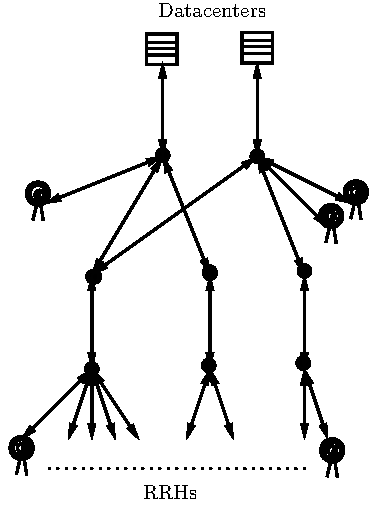
\includegraphics[scale=0.5]{extendendgraphgrey}\\
   \begin{itemize}
   \item Algorithms with theoretical guarantees for moderate load.
   \item FPT algorithm based on single processor scheduling.
   \end{itemize}
   \vspace{1cm}
\includegraphics[scale=0.5]{starfronthaul}
   \begin{itemize}
    \item Local search algorithms (hill climbing, simulated anealing) 
       \item Optimized Branch and bound: computes realistic instances.
   \end{itemize}
   \end{multicols}
\end{frame}



\end{section}
\begin{section}{Publications}

\begin{frame}{Publications}
	Published : 
   \begin{itemize}
    \item 2018 : Deterministic Scheduling of Periodic Messages for Cloud RAN. ICT 2018: 405-410
       \item 2019 : Deterministic Contention Management for Low Latency Cloud RAN over an Optical Ring. ONDM 2019: 479-491
   \end{itemize}
   
Submitted  / Finalisation : 
   \begin{itemize}
    \item Scheduling periodic messages on a shared link : STACS
       \item Deterministic Scheduling of Periodic Messages for Cloud RAN, Long paper : NETWORKS
   \end{itemize}
   \end{frame}
\end{section}

\begin{section}{Planning}

\begin{frame}{Planning}
\hspace{-1.3cm}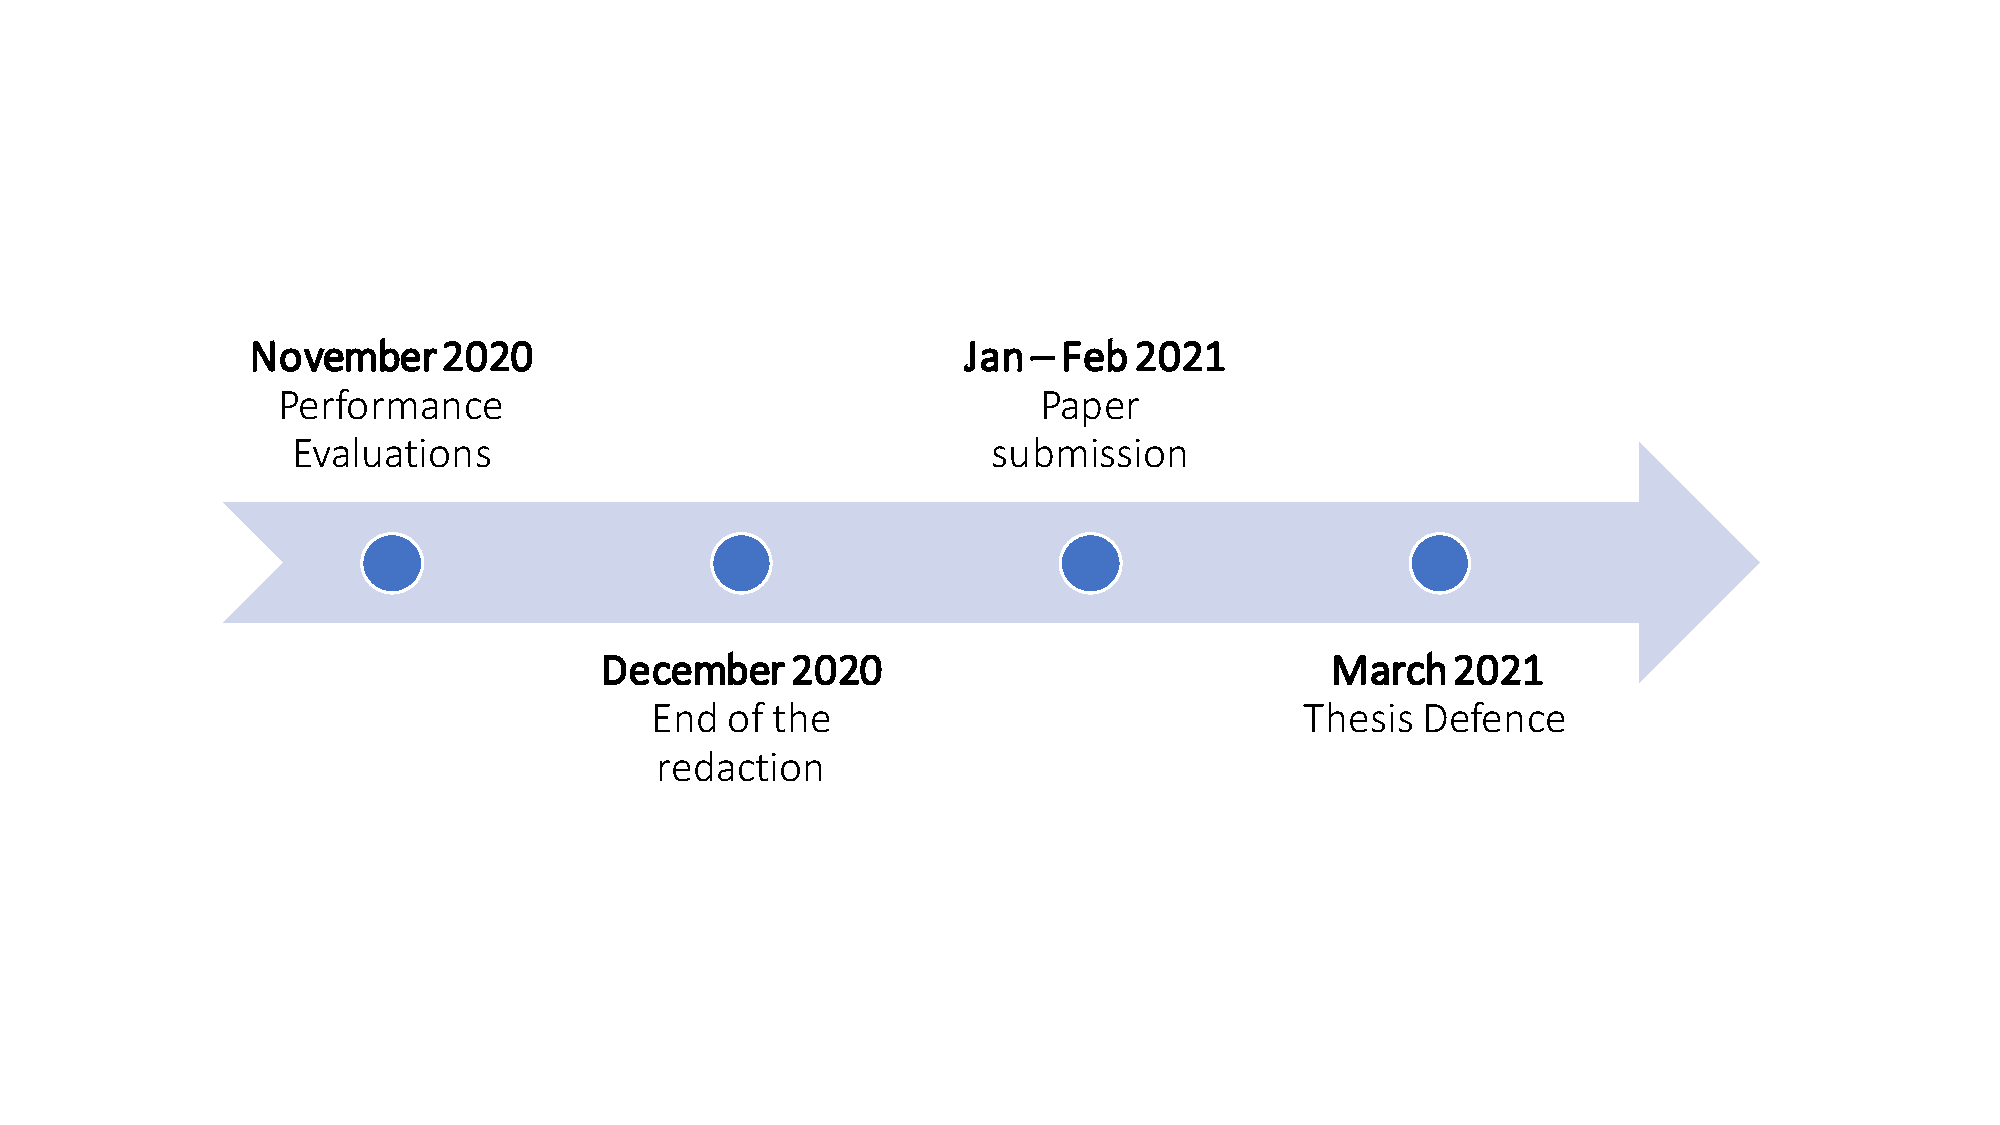
\includegraphics[scale=0.4]{timeline}

   \end{frame}
\end{section}


  \begin{frame}{Conclusion}

\begin{itemize}
 \item Research contract untill March 31.
 \item Training finalized.
\end{itemize}
 

\pause
\hspace{2cm}\huge{Thank you for your attention.}
  

\end{frame}




\end{document}
